\section{异步协作式调度}

\begin{frame}
    \frametitle{为何采用异步设计?}

    \begin{enumerate}
        \item 底层 IO 实现是异步的
              \begin{itemize}
                  \item SD 卡 IO 可以采用中断的形式实现
                  \item 网络设备一般可用 DMA
              \end{itemize}
        \item 统一内核与用户程序的调度
              \begin{itemize}
                  \item 用户程序在执行空转操作时可以通过系统调用让出执行权,那内核呢?
                  \item 同步内核需要手动插入调度点,而异步内核在每一个 await 处都是调度点
              \end{itemize}
        \item Rust 提供了足够好的异步编程支持
              \begin{itemize}
                  \item 没有强制要求使用特定的运行时,在 no-std 中也能使用
                  \item async / await 关键字提供了足够甜的语法糖
              \end{itemize}
    \end{enumerate}
\end{frame}

\begin{frame}
    \frametitle{异步内核实现要点}

    \begin{enumerate}
        \item 异步块设备与文件系统
              \begin{itemize}
                  \item 当所求数据在缓存中时,await 可以直接返回,性能几乎与同步版本相同
                  \item 当所求数据需要从块设备中读取时,await 会主动放弃当前 CPU 执行权
              \end{itemize}
        \item 异步管道与定时任务
              \begin{itemize}
                  \item 此类任务相比起 "轮询","通知" 显得更为自然而高效
                  \item 可以直接复用 waker 机制实现通知,复用异步调度器实现执行,无需额外代码
              \end{itemize}
        \item 异步睡眠锁
              \begin{itemize}
                  \item 自然地在锁竞争激烈时放弃竞争,进入睡眠
              \end{itemize}
        \item Fallback: \texttt{loop \{ yield().await \}}
              \begin{itemize}
                  \item 该方式可以模拟一切同步内核中的写法
                  \item 不断重新加入调度器末尾 + 放弃执行权,直到执行成功
              \end{itemize}
    \end{enumerate}
\end{frame}

\begin{frame}
    \frametitle{优势}

    在 IO 测试中 (\texttt{iozone}), 我们的内核取得了优异的成绩
    \begin{itemize}
        \item 异步实现能高效利用 CPU 执行时间,将尽可能多的 IO 请求并发执行
        \item 相对激进的缓存策略,尽可能填满板子的内存
    \end{itemize}

    \begin{figure}
        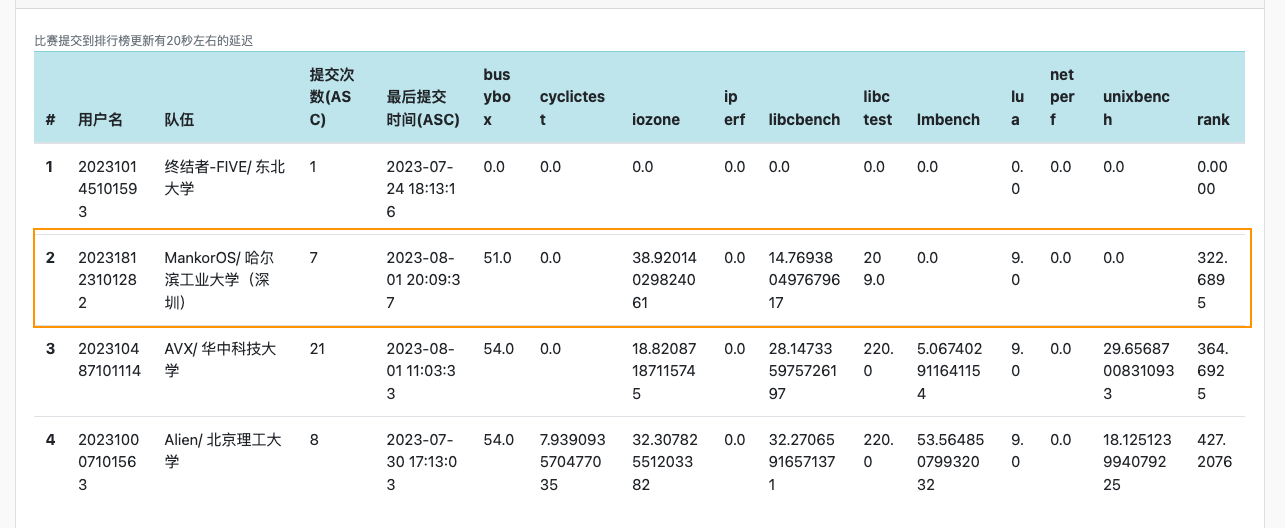
\includegraphics[width=.75\textwidth]{assets/leaderboard-final1.png}
    \end{figure}
\end{frame}

% \begin{frame}
%     \frametitle{不足}

%     \begin{enumerate}
%         \item 未能实现真正的异步 wait 系统调用
%               \begin{itemize}
%                   \item 目前仍然采用模拟同步的写法实现 wait
%                   \item 无法使得等待中的父进程 "睡熟", 性能与同步实现相比没有优势
%               \end{itemize}
%     \end{enumerate}
% \end{frame}

% 理论上这里还能加一页展望, 写写要是能突破 POSIX 限制, 异步内核能发展得怎么样